\documentclass[aspectratio=169]{beamer}
\usepackage{will_handley_beamer}
\usepackage{title_page}

% Commands
% --------
% - \arxiv{arxiv number}
% - \arxiv{<number>}            arxiv.org/abs/<number>
% - \oldarxiv{<arxiv number>}   arxiv.org/<number>
% - \doi{<doi>}                 doi.org/<doi>
% - \xkcd{<number>}             xkcd.com/<number>
% - \email{<email>}             <<email>>
% - \tthref{<website>}          <website>
% - \av[dist]{<quantity>}       <quantity>_{dist}
% - \student{<name>}{<detail>}{<photo>}

% Talk details
% ------------
% Figure generation scripts:
% - figures/lsbi_plot.py generates the sequential LSBI visualization (16 pages)
\title{\texttt{lsbi}: linear simulation based inference}
\date{June 19, 2025}

\begin{document}

\begin{frame}
    \titlepage
\end{frame}

\begin{frame}
    \frametitle{SBI: Simulation-based inference}
    \begin{columns}
        \column{0.5\textwidth}
        \begin{itemize}
            \item What do you do if you don't know \C[2]{$\mathcal{L}(D|\theta)$}?
            \item If you have a simulator/forward model $\theta \rightarrow D$
                defines an \C[2]{\emph{implicit} likelihood~$\mathcal{L}$}.
            \item Simulator generates samples from $\C[2]{\mathcal{L}(\cdot|\theta)}$.
            \item With a \C[1]{prior $\pi(\theta)$} can generate samples from \C[4]{joint distribution}~$\C[4]{\mathcal{J}(\theta,D)}=\C[2]{\mathcal{L}(D|\theta)}\C[1]{\pi(\theta)}$ (also called the \emph{unnormalised posterior})
            \item Task of SBI is take joint~$\C[4]{\mathcal{J}}$ samples and learn \C[0]{posterior $\mathcal{P}(\theta|D)$}
            \item Present state of the art achieves this using \emph{neural networks}
        \end{itemize}
        \column{0.5\textwidth}
        \includegraphics<1|handout:0>[page=1, width=\textwidth]{figures/sbi_parameter_estimation.pdf}%
        \includegraphics<2|handout:0>[page=2, width=\textwidth]{figures/sbi_parameter_estimation.pdf}%
        \includegraphics<3|handout:0>[page=3, width=\textwidth]{figures/sbi_parameter_estimation.pdf}%
        \includegraphics<4|handout:0>[page=4, width=\textwidth]{figures/sbi_parameter_estimation.pdf}%
        \includegraphics<5|handout:0>[page=5, width=\textwidth]{figures/sbi_parameter_estimation.pdf}%
        \includegraphics<6|handout:0>[page=6, width=\textwidth]{figures/sbi_parameter_estimation.pdf}%
        \includegraphics<7|handout:0>[page=7, width=\textwidth]{figures/sbi_parameter_estimation.pdf}%
        \includegraphics<8|handout:0>[page=8, width=\textwidth]{figures/sbi_parameter_estimation.pdf}%
        \includegraphics<9|handout:0>[page=9, width=\textwidth]{figures/sbi_parameter_estimation.pdf}%
        \includegraphics<10|handout:0>[page=10, width=\textwidth]{figures/sbi_parameter_estimation.pdf}%
        \includegraphics<11|handout:0>[page=11, width=\textwidth]{figures/sbi_parameter_estimation.pdf}%
        \includegraphics<12|handout:0>[page=12, width=\textwidth]{figures/sbi_parameter_estimation.pdf}%
        \includegraphics<13|handout:0>[page=13, width=\textwidth]{figures/sbi_parameter_estimation.pdf}%
        \includegraphics<14|handout:0>[page=14, width=\textwidth]{figures/sbi_parameter_estimation.pdf}%
        \includegraphics<15|handout:0>[page=15, width=\textwidth]{figures/sbi_parameter_estimation.pdf}%
        \includegraphics<16|handout:0>[page=16, width=\textwidth]{figures/sbi_parameter_estimation.pdf}%
        \includegraphics<17|handout:0>[page=17, width=\textwidth]{figures/sbi_parameter_estimation.pdf}%
        \includegraphics<18|handout:0>[page=18, width=\textwidth]{figures/sbi_parameter_estimation.pdf}%
        \includegraphics<19|handout:0>[page=19, width=\textwidth]{figures/sbi_parameter_estimation.pdf}%
        \includegraphics<20|handout:0>[page=20, width=\textwidth]{figures/sbi_parameter_estimation.pdf}%
        \includegraphics<21>[page=21, width=\textwidth]{figures/sbi_parameter_estimation.pdf}%
    \end{columns}
\end{frame}

\begin{frame}
    \frametitle{Why \textit{linear} SBI?}
    If neural networks are all that, why should we consider the regressive step of going back to linear versions?

    \begin{itemize}
        \item It is \textbf{pedagogically} helpful 
            \begin{itemize}
                \item separates general principles of SBI from the details of neural networks
                \item (particularly for ML skeptics)
            \end{itemize}
        \item It is \textbf{practically} useful
            \begin{itemize}
                \item for producing expressive examples with known ground truths
            \end{itemize}
        \item It is \textbf{pragmatically} useful
            \begin{itemize}
                \item competitive with neural approaches in terms of accuracy
                \item faster and more interpretable
            \end{itemize}
    \end{itemize}
\end{frame}

\begin{frame}
    \frametitle{Linear Simulation Based Inference}
    \framesubtitle{Mathematical setup and Bayesian Inference}
    \begin{columns}[t]
        \column{0.5\textwidth}
        \begin{itemize}
            \item Linear generative model $(m,M,C)$
                \[ D \sim \mathcal{N}(m + M \theta, C) \]
                where:
                \begin{description}
                    \item[$\theta$]: $n$ dimensional parameters
                    \item[$D$]: $d$ dimensional data
                    \item[$M$]: $d\times n$ transfer matrix
                    \item[$m$]: $d$-dimensional shift
                    \item[$C$]:  $d\times d$ data covariance
                \end{description}
            \onslide<2->{
            \item $k$ Simulations 
                \[ S=\{ (\theta_i,D_i): i=1,\ldots,k\} \]
            \item Define simulation statistics:
                \begin{description}
                    \item[$\bar\theta$] $= \tfrac{1}{k}\sum_i \theta_i$
                    \item[$\bar D$] $= \tfrac{1}{k}\sum_i D_i$
                    \item[$\Theta$] $=\tfrac{1}{k}\sum_i (\theta_i-\bar\theta)(\theta_i-\bar\theta)'$
                    \item[$\Delta$] $=\tfrac{1}{k}\sum_i (D_i-\bar D)(D_i-\bar D)'$
                    \item[$\Phi$] $=\tfrac{1}{k}\sum_i (D_i-\bar D)(\theta_i-\bar \theta)'$
                \end{description}
            }
        \end{itemize}

        \column{0.5\textwidth}
        \begin{itemize}
            \onslide<3->{
            \item We infer $(m,M,C)$ from simulations $S$. The likelihood is:
                \[P(\{D_i\}|\{\theta_i\}|m, M, C) = \prod_i \mathcal{N}(D_i|m+M\theta_i,C)\]
            }
            \onslide<4->{
            \item We use a conjugate prior $\pi$ on $(m,M,C)$ (with hyperparameters $\lambda_0, D_0, \theta_0, M_0, \Omega_0, \nu_0, \Psi_0$):
            \[
                \begin{array}{c}
                    \pi:
                    \left\{
                        \begin{aligned}
                            m&|M,C, \sim \mathcal{N}(D_0-M\theta_0, \tfrac{1}{\lambda_0}C), \\
                            M&|C, \sim \mathcal{MN}(M_0, C, \Omega_0^{-1}), \\
                            C &\sim \mathcal{W}^{-1}_{\nu_0}(\Psi_0)
                        \end{aligned}
                    \right.
                \end{array}
            \]
            }
            \onslide<5->{
            \item The posterior $\mathcal{P}$ for $(m,M,C)$ is: \student{toby_lovick.jpg}{Toby Lovick}{mathematical derivations}
            \[
                \mathcal{P}:
                \left\{
                    \begin{aligned}
                        m&|M,C,S \sim \mathcal{N}(m_\mathcal{P},C/\lambda_\mathcal{P}), \\
                        M&|C,S \sim \mathcal{MN}(M_\mathcal{P}, C,\Omega_\mathcal{P}^{-1}), \\
                        C&|S\sim \mathcal{W}^{-1}_{\nu_\mathcal{P}}(\Psi_\mathcal{P})
                    \end{aligned}
                \right.
            \]
            }
        \end{itemize}
    \end{columns}
\end{frame}

\begin{frame}
    \frametitle{LSBI vs Neural SBI: Explainability}
    \begin{columns}
        \column{0.6\textwidth}
        \textbf{Neural SBI challenges:}
        \begin{itemize}
            \item Black-box approximations
            \item Hyperparameter tuning required
            \item Saturation at $-5 < \log r < 5$
            \item Training instability
            \item Difficult convergence diagnostics
        \end{itemize}
        
        \vspace{0.3cm}
        \textbf{LSBI advantages:}
        \begin{itemize}
            \item Transparent mathematical foundation
            \item Self-tuning (no hyperparameters)
            \item Exact analytical solutions
        \end{itemize}

        \column{0.4\textwidth}
        \includegraphics[width=\textwidth]{figures/matrix_variate_distributions.jpg}
        
        \vspace{0.2cm}
        \footnotesize{Matrix-variate distributions provide exact analytical solutions}
    \end{columns}
\end{frame}

\begin{frame}
    \frametitle{Sequential LSBI}
    \begin{columns}
        \column{0.5\textwidth}
        \begin{itemize}
            \item Same model as before
            \item Mark the observed data~$D_\text{obs}$
            \item Fit a model using \texttt{lsbi}
            \item Evaluate the posterior (cheap as linear)
            \item Now use this posterior to pick $\{\theta_i\}$
            \item Generate $\{D_i\}$ from original simulator
            \item Fit \texttt{lsbi} to these
            \item Evaluate the new posterior
            \item Iterate until convergence
        \end{itemize}

        \column{0.5\textwidth}
        \includegraphics<1|handout:0>[width=\textwidth, page=1]{figures/lsbi_plot.pdf}%
        \includegraphics<2|handout:0>[width=\textwidth, page=2]{figures/lsbi_plot.pdf}%
        \includegraphics<3|handout:0>[width=\textwidth, page=3]{figures/lsbi_plot.pdf}%
        \includegraphics<4|handout:0>[width=\textwidth, page=4]{figures/lsbi_plot.pdf}%
        \includegraphics<5|handout:0>[width=\textwidth, page=5]{figures/lsbi_plot.pdf}%
        \includegraphics<6|handout:0>[width=\textwidth, page=6]{figures/lsbi_plot.pdf}%
        \includegraphics<7|handout:0>[width=\textwidth, page=7]{figures/lsbi_plot.pdf}%
        \includegraphics<8|handout:0>[width=\textwidth, page=8]{figures/lsbi_plot.pdf}%
        \includegraphics<9|handout:0>[width=\textwidth, page=9]{figures/lsbi_plot.pdf}%
        \includegraphics<10|handout:0>[width=\textwidth, page=10]{figures/lsbi_plot.pdf}%
        \includegraphics<11|handout:0>[width=\textwidth, page=11]{figures/lsbi_plot.pdf}%
        \includegraphics<12|handout:0>[width=\textwidth, page=12]{figures/lsbi_plot.pdf}%
        \includegraphics<13|handout:0>[width=\textwidth, page=13]{figures/lsbi_plot.pdf}%
        \includegraphics<14|handout:0>[width=\textwidth, page=14]{figures/lsbi_plot.pdf}%
        \includegraphics<15|handout:0>[width=\textwidth, page=15]{figures/lsbi_plot.pdf}%
        \includegraphics<16->[width=\textwidth, page=16]{figures/lsbi_plot.pdf}%
    \end{columns}
\end{frame}

\begin{frame}
    \frametitle{Cosmology Example: $\Lambda$CDM from CMB}
    \begin{columns}
        \column{0.52\textwidth}
        \begin{itemize}
            \item Apply LSBI to cosmic microwave background
            \item Cosmic-variance limited, temperature-only, full sky
            \item $n=6$ parameters, $d=2500$ data dimensions
            \item Sequential improvement around observed data
            \item Competitive with traditional methods
        \end{itemize}

        \column{0.48\textwidth}
        \includegraphics[page=11, width=\textwidth]{figures/cosmo_update.pdf}
    \end{columns}
\end{frame}

\begin{frame}
    \frametitle{\texttt{lsbi}: Code \& Implementation}
    \begin{itemize}
        \item \texttt{lsbi} is a pip-installable python package
        \item Extends \texttt{scipy.stats.multivariate\_normal}
            \begin{itemize}
                \item Vectorised distributions with broadcastable arrays
                \item \texttt{.marginalise(...)} and \texttt{.condition(...)} methods
                \item Built-in plotting functionality
            \end{itemize}
        \item Implements \texttt{LinearModel} class with interpretable methods:
            \begin{itemize}
                \item \texttt{.prior()}, \texttt{.likelihood(theta)}, \texttt{.posterior(D)}
                \item \texttt{.evidence()} - all return distributions
            \end{itemize}
        \item Also implements \texttt{MixtureModel} for nonlinear effects
        \item \arxiv{2501.03921} and \tthref{github.com/handley-lab/lsbi}
    \end{itemize}
\end{frame}

\begin{frame}
    \frametitle{Results \& Recent Work: \arxiv{2501.03921}}
    \framesubtitle{Performance, scaling, and key contributions}
    \begin{columns}
        \column{0.5\textwidth}
        \textbf{Key advantages:}
        \begin{itemize}
            \item Analytical solutions (no iterative training)
            \item Transparent mathematical operations
            \item Competitive with neural methods
            \item Faster than neural training, no GPU requirements
            \item Self-tuning (no hyperparameter search)
            \item Handles $n \approx 6$, $d \approx 2500$ problems
        \end{itemize}
        
        \textbf{Key contributions (\arxiv{2501.03921}):}
        \begin{itemize}
            \item Mathematical foundation using matrix-variate distributions
            \item Sequential refinement algorithm for nonlinear problems
            \item Comparison with neural approaches across test cases
            \item Open-source Python implementation
        \end{itemize}

        \column{0.5\textwidth}
        \textbf{Results demonstrate:}
        \begin{itemize}
            \item Competitive accuracy on standard benchmarks
            \item Significant computational speedup
            \item Enhanced interpretability 
            \item Pedagogical value for understanding SBI principles
        \end{itemize}
        
        \textbf{Available at:}
        \begin{itemize}
            \item \arxiv{2501.03921}
            \item \tthref{github.com/handley-lab/lsbi}
        \end{itemize}
        
        \vspace{0.5cm}
        \textbf{Master's student project} led to comprehensive framework paper with practical applications in cosmology and beyond.
    \end{columns}
\end{frame}

\begin{frame}
    \frametitle{Conclusions}
    \framesubtitle{\tthref{github.com/handley-lab/group}}
    \tikz[overlay,remember picture]
        \node[anchor=north east] (A) at ($(current page.north east)+(0,0)$) {
        \includegraphics[width=0.09\textheight]{people/adam_ormondroyd.jpg}%
        \includegraphics[width=0.09\textheight]{people/charlotte_priestley.jpg}%
        \includegraphics[width=0.09\textheight]{people/david_yallup.jpg}%
        \includegraphics[width=0.09\textheight]{people/dily_ong.jpg}%
        \includegraphics[width=0.09\textheight]{people/harry_bevins.jpg}%
        \includegraphics[width=0.09\textheight]{people/harvey_williams.jpg}%
        \includegraphics[width=0.09\textheight]{people/krish_nanavati.jpg}%
        \includegraphics[width=0.09\textheight]{people/metha_prathaban.jpg}%
        \includegraphics[width=0.09\textheight]{people/ming_yang.jpg}%
        \includegraphics[width=0.09\textheight]{people/namu_kroupa.jpg}%
        \includegraphics[width=0.09\textheight]{people/sam_leeney.jpg}%
        \includegraphics[width=0.09\textheight]{people/sinah_legner.jpg}%
        \includegraphics[width=0.09\textheight]{people/toby_lovick.jpg}%
        \includegraphics[width=0.09\textheight]{people/wei-ning_deng.jpg}%
        \includegraphics[width=0.09\textheight]{people/will_handley.jpg}%
        \includegraphics[width=0.09\textheight]{people/will_templeton.jpg}%
    };
    \begin{itemize}
        \item \textbf{lsbi} provides explainable alternative to neural SBI methods
        \item Separates SBI principles from ML implementation details  
        \item Competitive accuracy with interpretable mathematical foundation
        \item Available: \arxiv{2501.03921} and \tthref{github.com/handley-lab/lsbi}
        \item Future: realistic simulations, model comparison, importance sampling
    \end{itemize}
\end{frame}

\end{document}
